\chapter{Grundlagen}
\label{chap:grundlagen}

%\section{Analyse der Marsoberfläche}
%\label{sec:analysedermarsoberflache}

\section{Remote Sensing Instruments} % TODO ???
\label{sec:mars_images}

Von der Marsoberfläche existieren verschiedenste Arten von Aufnahmen für unterschiedliche Analysen. Dabei kommt es auf gewisse Parameter, wie \zB die aufgenommene Wellenlänge, den Winkel zur Oberfläche, die Auflösung, Brennweite, Ort der Aufnahme und viele weitere an, ob ein Bild zur Analyse einer gewissen Eigenschaft geeignet ist.

Für die hier genutzten Anwendungsfälle eignen sich Instrumente am besten, die sichtbares Licht aufnehmen. Diese sollten in Graustufen, in diesem Einsatzbereich also panchromatisch, aufgenommen sein, da die Farbe der Oberfläche deren Analyse hier wenig beeinflusst. Der Vorteil von Graustufenaufnahmen besteht darin, dass nur ein drittel des Speichers bei den Berechnungen benötigt wird.

Des weiteren sollten die Bilder eine vergleichsweise hohe Auflösung haben, damit auch kleinere Merkmale gut erkannt werden können, es sollten aber auch weite Aufnahmen sein, damit mit einem Datensatz ein Großteil der Oberfläche analysiert werden kann.

Außerdem eignen sich Fotos gut, die senkrecht zur Oberfläche entstanden sind, so dass diese nicht verzerrt erscheint.

Unter Berücksichtigung dieser Faktoren ergeben sich \ua zwei geeignete Instrumente:
Die \textit{Context Camera (CTX)} des \textit{Mars Reconnaissance Orbiters} der NASA \cite{malin_07} und die \textit{High Resolution Stereo Camera (HRSC)} des \textit{Mars Express Orbiters} der ESA \cite{hrsc}. Für die eigentlichen Analysen werden Aufnahmen der CTX genutzt, da sie einen Großteil der Oberfläche abdecken, während die panchromatischen Bilder der HRSC zur Evaluierung genutzt wurden, da mit ihnen schon mehrere andere Algorithmen getestet wurden.

\section{Convolutional Neural Networks}	% TODO MLP
\label{sec:cnn}

Neuronale Netze -- meist synonym mit Deep Learning genutzt -- werden oftmals als eine Weiterentwicklung oder Optimierung des maschinellen Lernens betrachtet: Statt einer Menge von Formeln, die die Approximation einer Funtion erlernen sollen, setzt man hier auf mehrere Schichten, auch Layers genannt, von vergleichsweise einfachen linearen Funktionen, um zur gewünschten Approximation zu kommen. \cite{hardesty_17}

In diesem Kontext wird ein Knoten, auch als Neuron bezeichnet. Ein typisches Neuron verarbeitet einen Eingabevektor indem es das Kreuzprodukt mit eben diesem Vektor und den verschiedenen Gewichtungen berechnet und anschließend einen Bias aufaddiert. Während das Netzwerk trainiert wird, passen die einzelnen Knoten diese zwei Vektoren, also die Gewichtungen und die Biasse an. Diese Gewichtungen sind anfangs zufällig bestimmt. \cite{hardesty_17, cs231n}

Die Aneinanderkettung dieser verschiedenen Schichten führt dazu, dass zwischen ihnen eine immer abstrahiertere Form der Eingabedaten entsteht, damit sind sie in ihrer Funktionsweise an die des menschlichen Gehirns angelehnt, welches sich auch aus einer Großzahl von hintereinandergeschalteten Neuronen zusammensetzt. % TODO Cite

Convolutional Neural Networks beschreiben eine Teilmenge der neuronalen Netze, in der die jeweilige Netzwerkarchitektur mindestens eine Convolutional Layer (auch Faltungsschicht genannt, \vgl Unterabschnitt~\ref{ssec:conv}) enthält. Die Nutzung dieser Convolutional Layer zieht fast immer die Nutzung einer Pooling Layer (Unterabschnitt~\ref{ssec:pooling}) mit sich. \cite{deeplearning_16}

Obwohl Convolutional Neural Networks theoretisch dazu geeignet sind die meisten Daten mit einer gitterähnlichen Struktur zu verarbeiten, erfreuen sie sich im Bereich der Bilddatenanalyse der größten Beliebtheit. \cite[Kap.~9]{deeplearning_16} Eine wichtige Ursache für diese Beliebtheit liegt \bspw in dem Erfolg bei dem Bild-Klassifizierungs-Wettbewerb \textit{ImageNet}. Während dort im Jahr 2011 die Gewinnergruppe mit klassischen Klassifizierungsalgorithmen einen Top-5-Score von $74,3\%$ erzielt hat, wurden im Jahr 2012 mit einem CNN erstmals ein Wert von $83,6\%$ erreicht. Von diesem Punkt an wurde die Bestenliste der darauffolgenden Jahre durch Convolutional Neural Networks dominiert. \cite[Kap.~1]{deeplearning_18}

% TODO Add Automonous Driving for segmentation problems

% TODO "Normal Network Architecture%

Die Architektur eines typischen, einfachen Convolutional Neural Networks ist wie folgt \cite{cs231n}:

\begin{multline*}
\mathrm{INPUT}\rightarrow\mathrm{CONVOLUTIONAL}\rightarrow\mathrm{ACTIVATION}\\\rightarrow\mathrm{POOLING}\rightarrow\mathrm{FULLYCONNECTED}
\end{multline*}

Da CNNs primär auf Bilddateien angewandt werden, wird von diesem Punkt an von einer Bilddatei als Eingabe (INPUT) ausgegangen. Hier beschreiben die ersten beiden Dimensionen die Breite und Höhe, während die dritte Dimension die Farbwerte für den jeweiligen Pixel angibt.

\subsection{Konvolution}
\label{ssec:conv}

Die Konvolution ist eine mathematische Operation auf zwei Funktionen $f(x)$ und $g(y)$, die eine dritte Funktion, die Konvolution $s = f*g$ ergibt, welche beschreibt, wie sich die Verläufe der beiden Funktionen beeinflussen:

\begin{equation}
s(x) = (f*g)(x) = \int_{-\infty}^{\infty} f(y)g(x-y)dy
\end{equation}

In einem Großteil der Anwendungsfälle der Konvolution bestehen die Eingabefunktionen aus einer Eingabefunktion $x$ und einem Kernel $w$, die Ausgabe ist die Merkmalsdimension. In einer praktischen Anwendung wären dies \bspw Messwerte $x(t)$ in Abhängig von der Zeit und einer Gewichtungsfunktion $w(a)$ in Abhängigkeit des Alters der Messung. Für ungültige Zeiten (\bspw Zukunft) gilt $w=0$ \cite[Kap.~9]{deeplearning_16}:

\begin{equation}
s(t) = (x*w)(t) = \int_{-\infty}^{\infty} x(a)w(t-a)da
\end{equation}

Unter der Annahme, dass die Eingabewerte nicht stetig sondern diskret sind (\bspw zeitliche Messwerte in regelmäßigen Abständen) ergibt sich vereinfacht \cite[Kap.~9]{deeplearning_16}:

\begin{equation}
s(t) = (x*w)(t) = \sum_{a=-\infty}^{\infty}x(a)w(t-a)
\end{equation}

Diese Funktion lässt sich für zweidimensionale Eingabedaten, wie \zB eine Bilddatei $I$ und einen zweidimensionalen Kernel $K$ erweitern \cite[Kap.~9]{deeplearning_16}:

\begin{equation}
S(i,j) = (I*K)(i,j) = \sum_{m}\sum_{n}I(m,n)K(i-m,j-n)
\end{equation}

Eine alternative Betrachtungsweise dieser Formel basiert auf dem Hadamard-Produkt. Angenommen, es existieren eine Matrix $I\in\mathbb{R}^{2}$ und eine Matrix $K\in\mathbb{R}^{m\times n}$.

Sei Matrix $H$ definiert als Hadamard-Produkt aus und $K$ und $I'=I_{x, y}$ mit $x\in[i-m,i]$ und $y\in[j-n,j]$.
Dann gilt $S(i,j)=\sum_{h\in H}h$

Diese Formel gilt allerdings nur für Eingabebilder mit nur einem Farbwert pro Pixel, also Graustufenbilder. Für ein Bild mit beliebig vielen Farbwertsdimensionen gilt:

\begin{equation}
S(i,j) = (I*K)(i,j) = \sum_{m}\sum_{n}\sum_{o}I(m,n,o)K(i-m,j-n,o)
\end{equation}

Es ist zu beachten, dass der Farbvektor immer komplett verarbeitet wird, und nicht nur ein Teilausschnitt wie bei Höhe und Breite.

\subsection{Convolutional Layer}
\label{ssec:convlayer}

Klassische Schichten von neuronalen Netzen nutzen Matrixmultiplikationen der kompletten Eingabe mit einer Parametermatrix um ihre Ausgaben zu berechnen, \dh jeder einzelne Ausgabewert entsteht aus einer Berechnung basierend auf jedem einzelnen Eingabewert. Obwohl diese Taktik in vielen Einsatzbereichen gut Funktioniert, stößt sie insbesondere bei der Bilddatenanalyse an ihre Grenzen, da sie nicht gut skaliert. \cite{cs231n} So benötigt eine Convolutional Layer zum Erkennen eines Merkmals nur einen Kernel mit einer Anzahl von meistens unter $\SI{100}{\pixel}$. \cite{deeplearning_16} Ein weiterer Pluspunkt besteht daraus, dass durch Convolutional Layers bestimmte Merkmale von unterschiedlichen Stellen der Eingabe extrahiert werden können, wie später beschrieben.

\begin{figure}[H]
	\centering
	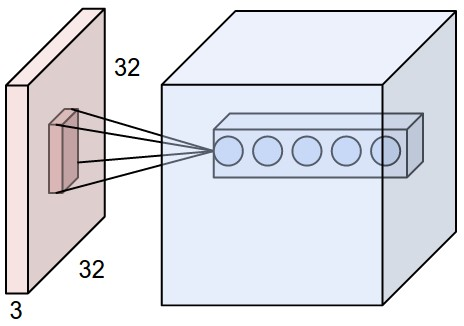
\includegraphics[width=0.4\textwidth,keepaspectratio]{images/cs231n/convolutional.jpg}
	\caption{Funktionsweise der Konvolutions-Schicht, aus \cite{cs231n}}
	\label{fig:convolutional}
\end{figure}

Eine konvolutionelle Schicht besteht aus einer Menge von Neuron, welche die Eingabe über den eben beschriebenen Konvolutionsoperator $S(i,j)$ auf genau ein Merkmal untersuchen. Daraus folgt, dass die Anzahl der Neuronen in eben dieser Schicht gleich der Größe der entstehenden Merkmalsdimension ist. (\vgl \figurename~\ref{fig:convolutional})

Hierbei gilt es zu beachten, dass der Konvolutionsoperator für alle Werte $i$ und $j$ der Eingabedimensionen aufgerufen wird, so dass die Höhe und Breite der Ausgabe (bis auf einige Ausnahmen) identisch zu denen der Eingabe ist.
Des Weiteren ist der Kernel pro Neuron konstant. Dies hat \ua zur Folge, dass das gleiche Merkmal an verschiedenen Stelle in der Eingabe erkennen kann.

Erhält eine konvolutionelle Schicht mit 12 Neuronen also \bspw ein RGB-Eingabebild der Größe $\SI{64}{\pixel}\times\SI{64}{\pixel}$, so erzeugt es mit einem Stride von $1$ als Ausgabe eine dreidimensionale Matrix der Größe $64\times64\times12$, jede der Schichten der dritten Dimensionen deutet auf das Vorhandensein eines speziellen Merkmals an einer gewissen Stelle im Eingabebild hin.

Das Hinzufügen von konvolutionellen Schichten führt allerdings zu mehr Hyperparametern, die optimiert werden können \cite{cs231n}:
\begin{itemize}
	\item Die Dimensionen des Kernels $k_1$ und $k_2$ (obwohl dieser fast immer quadratisch ist, oftmals $3$)
	\item Die Anzahl der Neuronen/der Merkmalsdimensionen
	\item Die Größe der Strides (die Schrittweite). Hier wird von einem Wert von $1$ ausgegangen, was die Größe der Ausgabe nicht verändert.
	\item Das Padding, also wie sich die Konvolution an den Rändern der Eingabedaten verhält. Hier wird von Zero-Padding ausgegangen, dies hat zur Folge, dass es die Größe der Ausgabe unverändert lässt.
\end{itemize}

\subsection{Activation Layer}
\label{ssec:activation}

Auf eine konvolutionelle Schicht folgt fast immer eine Aktivierungsschicht. Diese werden dazu genutzt um eine gewisse Nicht-Linearität in den Verlauf des neuronalen Netzes einzuführen. Nicht-Linearität ist in vielen neuronalen Netzen notwendig, da die von ihnen zu lösenden Probleme keine Linearen sind. \cite[Kap.~6]{deeplearning_16}

Selbst wenn nach der letzten Schicht eines mehrschichtigen neuronalen Netzes eine Aktivierungsschicht hinzugefügt werden würde, hätte dies zur Folge, dass die vorherigen Schichten wie eine einzige lineare Schicht agieren, was keine Vorteile gegenüber einer einzigen Schicht hat. Somit sollte jede einzelne Schicht von einer Aktivierungsschicht gefolgt sein, um verschiedenste, komplizierte Zusammenhänge zwischen Ein- und Ausgabedaten besser approximieren zu können. \cite[Kap.~3]{deeplearning_18}

In \figurename~\ref{fig:activations} sind drei der am meisten Verbreiteten Aktivierungsfunktionen zu sehen.

\begin{figure}[h!]
	\captionsetup[subfigure]{labelformat=empty}
	\begin{subfigure}{0.33\textwidth}
		\centering
		\subcaption{ReLU: $f(x)=\mathrm{max}\{0,x\}$}
		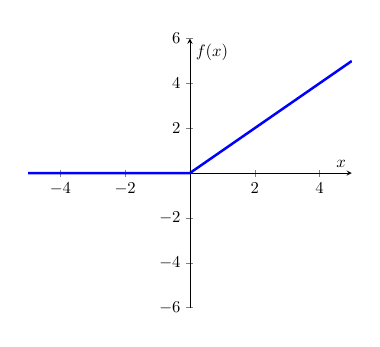
\begin{tikzpicture}[scale=0.6]
			\begin{axis}[
				axis lines = middle,
				xlabel = {$x$},
				ylabel = {$f(x)$},
				domain=-5:5,
				]
				\addplot[draw=blue,domain=-5:5,line width=1.5]{max(0,x)};
				\addplot[draw opacity=0,domain=-5:5]{1.2*x};
			\end{axis}
		\end{tikzpicture}
	\end{subfigure}
	\begin{subfigure}{0.32\textwidth}
		\centering
		\subcaption{Sigmoid: $f(x)={1}/{(1+e^{-x})}$}
		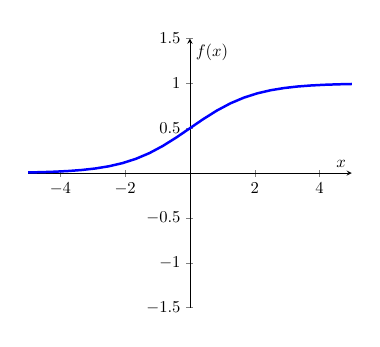
\begin{tikzpicture}[scale=0.6]
			\begin{axis}[
				axis lines = middle,
				xlabel = {$x$},
				ylabel = {$f(x)$},
				domain=-5:5,
				]
				\addplot[draw=blue,domain=-5:5,line width=1.5]{1/(1+e^(-x))};
				\addplot[draw opacity=0,domain=-5:5]{0.3*x};
			\end{axis}
		\end{tikzpicture}
	\end{subfigure}
	\begin{subfigure}{0.33\textwidth}
		\centering
		\subcaption{tanh: $f(x)=tanh(x)$}
		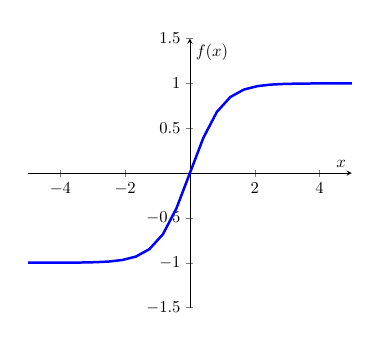
\begin{tikzpicture}[scale=0.6]
			\begin{axis}[
				axis lines = middle,
				xlabel = {$x$},
				ylabel = {$f(x)$},
				domain=-5:5,
				]
				\addplot[draw=blue,domain=-5:5,line width=1.5]{tanh(x)};
				\addplot[draw opacity=0,domain=-5:5]{0.3*x};
			\end{axis}
		\end{tikzpicture}
	\end{subfigure}
	\caption{Drei Aktivierungsfunktionen}
	\label{fig:activations}
\end{figure}

\subsection{Pooling Layer}
\label{ssec:pooling}

\begin{wrapfigure}{r}{0.38\textwidth}
	\centering
	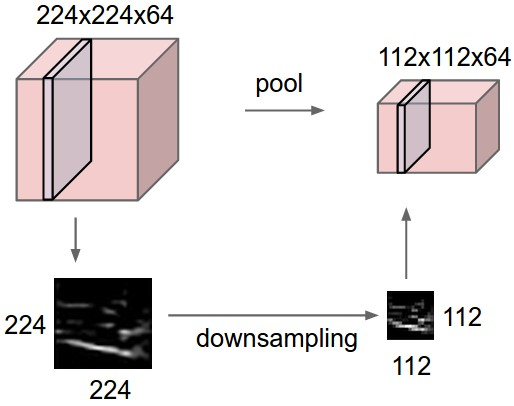
\includegraphics[width=0.37\textwidth,keepaspectratio]{images/cs231n/pool.jpg}
	\captionsetup{format=plain}
	\caption{Funktionsweise der Pooling-Layer, aus \cite{cs231n}}
	\label{fig:pooling}
\end{wrapfigure}

Konvolutionelle Schichten in neuronalen Netzen können die selben Merkmale von unterschiedlichen Stellen extrahieren. Die Position, an der diese Merkmale erkannt wurden, werden auch an die nächste Schicht weitergegeben, \dahe kleine Veränderungen an der Position eines Merkmals führen zu einer veränderten Merkmalsdimension. \cite{brownlee_19} Dies kann insbesondere beim Einsatz von mehreren konsekutiven Convolutional Layers zu einer erhöhten Störanfälligkeit führen, deshalb wird oftmals eine Pooling-Layer dazu eingesetzt, das resultierende Netzwerk invariant zu einzelnen Merkmalspositionen zu machen. \cite{deeplearning_16}

Ein weiteres Problem des Einsatzes von ausschließlich konvolutionellen Schichten besteht daraus, dass sie schnell zu einem hohen Anstieg der Parameterzahl im Netzwerk führen können: Jede neue Schicht erzeugt einen weiteren Datenwürfel der Größe $H\times W\times F$, wobei $H$ und $W$ die Höhe und Breite des Eingabebildes, und $F$ die Größe der Merkmalsdimension ist. Alle diese Werte werden im Training des neuronalen Netzes optimiert, was zu Performanceeinbüßungen führt. \cite{cs231n}

Die Pooling-Schicht verarbeitet alle Merkmalsdimensionen ihrer Eingabe unabhängig voneinander.

Für jede Merkmalsdimension überlauft der rezeptive Bereich -- ähnlich zur Konvolutions-Schicht -- die jeweilige Schicht des Würfels in Höhe und Breite, und berechnet je nach Pooling-Art einen Wert, welcher als positionsabhängige Ausgabe weitergeleitet wird. Dieser Prozess ist in \figurename~\ref{fig:pooling} anschaulich dargestellt.

Er besitzt zwei Hyperparameter: Die Stride (Schrittweite) $S$ und die eigentliche Größe $F_1\times F_2$. \cite{cs231n}

\begin{figure}[H]
	\centering
	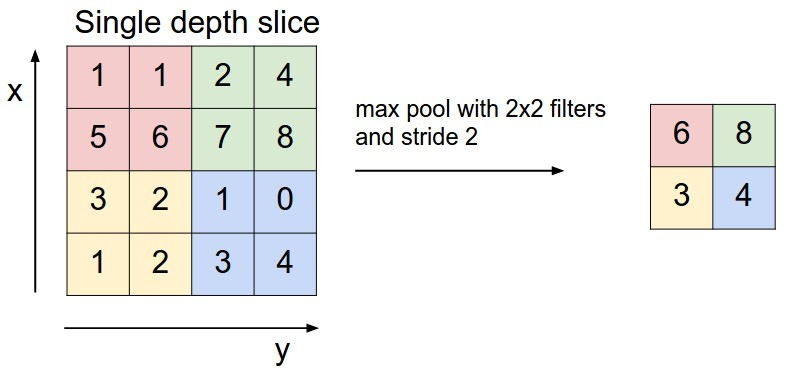
\includegraphics[width=0.5\textwidth,keepaspectratio]{images/cs231n/maxpool.jpg}
	\captionsetup{format=plain}
	\caption{Max-Pooling anhand eines Beispiels, aus \cite{cs231n}}
	\label{fig:maxpooling}
\end{figure}

Beim Max-Pooling übernimmt die Poolingoperation den maximalen Wert des von ihr überdeckten Eingabebereiches. (\vgl \figurename~\ref{fig:maxpooling})

\subsection{Batch Normalization}
\label{ssec:bn}

\subsection{Loss Function}
\label{ssec:loss}

Das Ziel eines neuronalen Netzes ist es, den Loss, also die Verlustfunktion, welche beschreibt wie weit die berechneten Werte von den im Training zu erzielenden Werten, in jeder Iteration weiter zu minimieren.

\subsection{Backpropagation}
\label{ssec:backpropagation}